\documentclass{article}
\usepackage{tikz}
\usetikzlibrary{arrows.meta,positioning,shapes.geometric,fit,calc}
\begin{document}
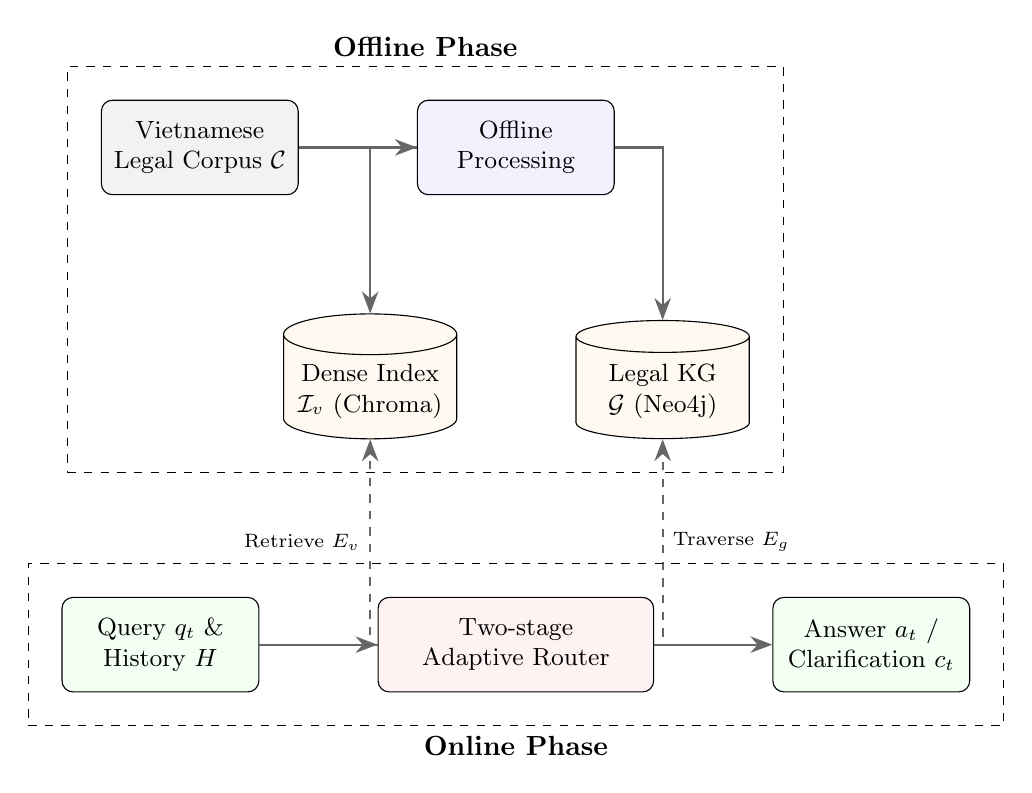
\begin{tikzpicture}[
    node distance=1.5cm and 1cm,
    box/.style={draw, rectangle, rounded corners, minimum width=2.5cm, minimum height=1.2cm, align=center, fill=blue!5, font=\small},
    db/.style={draw, cylinder, shape border rotate=90, aspect=0.25, minimum width=2.2cm, minimum height=1.5cm, align=center, fill=orange!5, font=\small},
    arrow/.style={-{Stealth[scale=1.2]}, thick, draw=gray!80!black},
    dashed_arrow/.style={-{Stealth[scale=1.2]}, thick, dashed, draw=gray!80!black}
]
    % Databases (center)
    \node[db] (chroma) {Dense Index \\ $\mathcal{I}_v$ (Chroma)};
    \node[db, right=1.5cm of chroma] (neo4j) {Legal KG \\ $\mathcal{G}$ (Neo4j)};
    
    % Offline
    \node[box, above=1.5cm of chroma, xshift=1.85cm] (offline) {Offline \\ Processing};
    \node[box, left=1.5cm of offline, fill=gray!10] (corpus) {Vietnamese \\ Legal Corpus $\mathcal{C}$};
    
    \draw[arrow] (corpus) -- (offline);
    \draw[arrow] (offline) -| (chroma);
    \draw[arrow] (offline) -| (neo4j);
    
    % Online
    \node[box, below=2cm of chroma, xshift=1.85cm, fill=red!5, minimum width=3.5cm] (router) {Two-stage \\ Adaptive Router};
    \node[box, left=1.5cm of router, fill=green!5] (query) {Query $q_t$ \& \\ History $H$};
    \node[box, right=1.5cm of router, fill=green!5] (output) {Answer $a_t$ / \\ Clarification $c_t$};
    
    \draw[arrow] (query) -- (router);
    \draw[arrow] (router) -- (output);
    
    \draw[dashed_arrow] (router) -| (chroma) node[near end, left, font=\scriptsize] {Retrieve $E_v$};
    \draw[dashed_arrow] (router) -| (neo4j) node[near end, right, font=\scriptsize] {Traverse $E_g$};
    
    % Grouping
    \node[draw, dashed, inner sep=12pt, fit=(corpus)(offline)(chroma)(neo4j), label={[font=\bfseries]above:Offline Phase}] (offline_box) {};
    \node[draw, dashed, inner sep=12pt, fit=(query)(router)(output), label={[font=\bfseries]below:Online Phase}] (online_box) {};
\end{tikzpicture}
\end{document}
